\chapter{Teoría de la Complejidad Computacional}\label{ch:teoría-de-la-complejidad-computacional}
Consideremos 2 tipos de recursos:
\begin{itemize}
  \item \textbf{Tiempo:} tiempo de ejecución o número de pasos base.
  \item \textbf{Espacio:} recursos de memoria utilizados.
\end{itemize}

\section{La Máquina de Turing y medida de la Complejidad}
El tiempo de ejecución de Máquina de Turing es la función $T(n): N \rightarrow N$, donde T(n) es el número máximo de pasos que una MT utiliza para realizar el cómputo para entrada de tamaño n.

Complejidad Computacional: se refiere a la complejidad de los problemas.
\begin{itemize}
  \item Se toma la peor instancia
  \item Se utiliza la Cota Superior  Asintótica: O(g)
\end{itemize}

La principal herramienta para comparar problemas y clasificarlos:
\begin{itemize}
  \item Desde el punto de vista de la computabilidad
  \item Desde el punto de vista de la complejidad computacional
\end{itemize} 

\section{Reducción entre problemas}
Dado dos Lenguajes A y B, y una función $f: \Sigma^* \rightarrow \Sigma^*$.

f es una transformación del lenguaje universal del problema A al lenguaje universal del problema B. Se dice que \textbf{A es reducible a B}, bajo f si:

$$\begin{matrix}
  \forall w \in A \Leftrightarrow f(w)\in B \\ 
  A \leq_f B
\end{matrix}$$

\textbf{Reducción:} transformar un problema en otro. Transformar toda instancia de un problema en instancias de otro problema.

Intuitivamente:
\begin{itemize}
  \item es una manera de convertir un problema a otro problema, de tal manera que la solución al segundo problema se puede utilizar para resolver el primer problema.
  \item ''Si el problema A es reducible al problema B, entonces la solución al problema B se
  puede utilizar para resolver el problema A''
\end{itemize}

Formalmente:
\begin{itemize}
  \item Si el coste de Reducir A en B, es decir, el proceso de transformar una instancia de A en una instancia de B, es de orden polinómico (o menor) se puede afirmar que:
  \begin{itemize}
    \item Resolver A no puede ser más complejo (''harder'') que resolver B. Es decir, resolver A a lo sumo es tan complejo de resolver como B.
    \item Resolver B al menos es tan complejo como resolver A
    \item Estas dos afirmaciones se expresan así: $A \leq B$
  \end{itemize}
  \item Reducir el problema A al problema B en tiempo polinómico implica que la reducción se lleva a cabo con una función cuyo $T(n)=O(n^k)$, $A \leq_p B$
  \item Si $A \leq_p B$ y $B \leq_p A$ son igual de difíciles.
\end{itemize}

\section{Clases de Problemas}
Tiempo
\begin{itemize}
  \item Clase P
  \item Clase NP
  \item Clase NP-Completo 
  \item Clase NP-Hard
\end{itemize}

Espacio
\begin{itemize}
  \item Clase P-Space
  \item Clase NP-Space
\end{itemize}

\textbf{TIME(f(n)):} Conjunto de problemas de decisión que se pueden resolver mediante una Máquina de Turing Determinista con coste $O(f(n))$.

\textbf{NTIME(f(n)):} Problemas de decisión que se pueden resolver mediante una Máquina de Turing NO Determinista con coste $O(f(n))$.

Lo que una MTD puede resolver en Time($2^n$), una MTND  lo puede resolver en menor tiempo NTIME(n). Pero no al revés, porque no sabemos cuánto más tardara. 

\subsection{Complejidad Temporal}
\subsubsection{Clase P}
Problemas (Lenguajes) decidibles por una MT Determinista (de una sola cinta) en TIEMPO POLINÓMICO. $P= \bigcup_k TIME(n^k)$
\begin{itemize}
  \item Time($n$), Time($n^2$), ..., Time($n^k$)
\end{itemize}

La clase P contiene todos los problemas decibles por un algoritmo que cuyo coste computacional (tiempo) es de orden polinómico con respecto al tamaño de la entrada (n).

''P se corresponde con la clase de problemas que se pueden resolver desde un punto de vista realista/práctico en un computador''

La mayoría de los problemas corrientes pertenecen a la clase P: Ordenación, Búsqueda, Operaciones con vectores.

“La clase P es robusta”
\begin{itemize}
  \item La clase P es invariante (i.e. robusta) para todos los modelos de computación que son polinómicamente equivalentes a la MT Determinista de una sola cinta.
  \item Los problemas en P permanecen en P aunque se cambie el modelo de computación.
\end{itemize}

Ejemplos de problemas en P:
\begin{itemize}
  \item Si existe un camino entre dos puntos en un grafo
  \item Si x e y son coprimos
  \item Si x es primo (AKS lo demuestra)
\end{itemize}

\subsubsection{Clase NP}
Problemas (Lenguajes) decidibles por una MT NO Determinista (de una sola cinta) en TIEMPO POLINÓMICO. $NP= \bigcup_k NTIME(n^k)$
\begin{itemize}
  \item Time($n$), Time($n^2$), ..., Time($n^k$)
  \item NTime($n$), NTime($n^2$), ..., NTime($n^k$)
\end{itemize}

Es decir, problemas para los que existe una MT NO DETERMINISTA que da solución parándose (da una respuesta sea cual sea la entrada) en TIEMPO POLINÓMICO.

NP es la clase de \textbf{lenguajes que tienen un verificador en tiempo polinómico}. Que no se conozca, no quiere decir, no exista uno en tiempo polinómico.

Todo P es NP, $P \leq NP$, pero no se ha podido demostrar que sean el mismo conjunto, por ahora $P \subset NP$.

Podemos \textbf{evitar la fuerza bruta para conseguir soluciones de muchos problemas} en tiempo polinómico. Pero para \textbf{otros problemas no se conocen soluciones en tiempo polinómico}. No se sabe si se podrán conseguir, podría suceder que estos \textbf{problemas fueran intrínsecamente difíciles}.

Si un problema \textbf{no es NP, no es TD}.

Lo primero y más fácil que podemos utilizar para saber si pertenece a NP es hace un verificador, y si este lo hace en tiempo polinómico.

El segundo paso es ver si este se puede resolver con una MT ND.

\subsubsection{Verificabilidad}
Verificador V para un lenguaje L: $L=\{w / V \textit{ acepta } <w,c> \textit{ para alguna palabra }c\}$
$$w \in L \Rightarrow \exists c \in \Sigma^*. V \textit{ acepta } <w, c>$$
\begin{itemize}
  \item \textbf{Verificador:} Es un algo que permite ver si una instancia/cadena cumple el problema o no, pero no lo resuelve. Dice si la solución es buena o no. 
  
  El verificador asociado a un problema debe tener para cada una de las palabras de dicho problema (w) una cadena c llamada certificado que hace que termine el verificador en un estado de aceptación. Para aquella que no sean del lenguaje las rechazara, no habrá un c.
  \item \textbf{Certificador:} Cadena que se asocia a una salida w que recibe el verificador que ayuda a saber si la solución pertenece al lenguaje.
\end{itemize}

Si V se ejecuta en tiempo polinómico, V es un verificador en tiempo polinómico, y L es polinómicamente verificable

NP es la clase de lenguajes que tienen verificadores en tiempo polinómico.

Encontrar un verificador es más sencillo que resolver el problema, este solo dice si es una buena solución o no resuelve el problema.

\subsubsection{P vs. NP}
\textbf{P} es la clase de lenguajes en los que la pertenencia de una palabra puede ser \textbf{decidida rápidamente}. (reconocer/aceptar)

\textbf{NP} es la clase de lenguajes en los que la pertenencia puede ser \textbf{verificada rápidamente}. (verificar)

\subsubsection{Clase EXPTIME}
$EXPTIME= \bigcup_k TIME(2^{n^k})$

Todos los conjuntos exponenciales. $NP \leq EXPTIME$

\subsubsection{Clase NP-Completo}
Un problema de decisión $p\in NP-Completo$ si y solo si:
\begin{itemize}
  \item $p \in NP$
  \item $\forall q \in NP$ existe una reducción de q en p. Es decir, existe una transformación f de coste polinómico de q en p, tal que $q \leq_p p$
\end{itemize}

Los problemas NPC se pueden reducir entre ellos.

Todos los problemas de NP se pueden reducir en tiempo polinómico en NP-Completo. De esta manera se puede demostrar que un problema pertenece a NP-Completo, si se puede reducir en tiempo polinómico un problema NP-Completo a este.
\begin{itemize}
  \item Tenemos los problemas $p$ y $ q\in NP-Completo$, por lo que si $q \leq_p p$ entonces $p \in NP-Completo$.
  \item Ejem. Como el Buscaminas (Minesweeper) es más difícil que SAT y sabemos que SAT es NP-Completo entonces Buscaminas es NP-Completo.
\end{itemize}

Formas de resolver problemas en tiempo razonable:
\begin{itemize}
  \item \textbf{Aproximaciones:} Un algoritmo que rápidamente encuentra una solución no necesariamente óptima, pero dentro de un cierto rango de error.
  
  En algunos casos, encontrar una buena aproximación es suficiente para resolver el problema, pero no todos los problemas NP-completos tienen buenos algoritmos de aproximación.
  \item \textbf{Probabilístico:} Un algoritmo probabilístico obtiene en promedio una buena solución al problema planteado, para una distribución de los datos de entrada dada.
  \item \textbf{Casos particulares:} Cuando se reconocen casos particulares del problema para los cuales existen soluciones rápidas.
  \item \textbf{Heurísticas:} Un algoritmo que trabaja razonablemente bien en muchos casos. En general son rápidos, pero no existe medida de la calidad de la respuesta.
  \item \textbf{Meta heurística (Computación evolutiva, Algoritmo Genético):} Algoritmos que mejoran las posibles soluciones hasta encontrar una que posiblemente esté cerca del óptimo. Tampoco existe forma de garantizar la calidad de la respuesta.
\end{itemize}

3SAT es NP-Completo, pero 2SAT no.

\subsubsection{3SAT $\leq$ K-Clique}
K-Clique sabemos que es NP, vamos a demostrar si es NP-Completo.
$$\textit{3SAT} \leq \textit{K-Clique}$$

Cada literal es un vértice del clique. Con 3 cláusulas tenemos 9 literales, por tanto, 9 vértices. $\phi=(x\vee y \vee z) \wedge (x\vee x \vee \overline{y}) \wedge \dots$

Entonces se hacen todas las conexiones posibles siguiendo:
\begin{itemize}
  \item No se conectan literales en la misma cláusula.
  \item Un literal no se conecta con su opuesto. $y \; e\; \overline{y}$
\end{itemize}

La solución será aquella que haga True todas las cláusulas, que coincide con un clique en el grafo que hemos generado.

\begin{enumerate}
  \item $w\in \textit{3SAT} \rightarrow f(w)\in \textit{K-Clique}$ y $f(w)$ se puede hacer en tiempo polinómico.
  
  Supongamos que $\phi$ tiene una asignación satisfacible de literales.
  \begin{itemize}
    \item Entonces un literal por lo menos en cada cláusula debe tener valor de verdadero (ya que en cada cláusula hay solo disyunciones)
    \item En cada cláusula representada en el grafo seleccionamos un solo vértice con valor de verdadero. Habremos seleccionado k vértices que estarán interconectados en CLIQUE.
  \end{itemize}
  \item $f(w)\in \textit{K-Clique} \rightarrow w \in \textit{3SAT}$
  
  Supongamos que el grafo tiene un k-clique
  \begin{itemize}
    \item No habrá vértices en el grafo que correspondan a la misma cláusula de una forma normal conjuntiva de k cláusulas, ya que hemos seleccionado solo un vértice por cláusula: cada cláusula correspondiente contiene un vértice en el grafo.
    \item Asignemos valores a los literales para que cada uno de los que etiquetan un nodo en el CLIQUE sea verdadero.
  \end{itemize}
\end{enumerate}
\pagebreak

\subsubsection{Clase NP-Hard}
Un problema de decisión $h \in \textit{NP-Hard}$ si y solo si:
\begin{itemize}
  \item $\forall q \in NP$, existe una reducción de q en h. Es decir, existe una transformación f de coste polinómico de q en h tal que $q \leq_p h$
\end{itemize}

Los NP-Hard pueden reducir los NP sin ser NP, siendo NTD.

Todos los NPC son NPH, $\textit{NPC}=\textit{NP} \cap \textit{NP-Hard}$, pero no todos los NPH son NPC porque no están en NP.

Es el conjunto de los problemas de decisión que contiene los problemas h tales que todo problema q en NP puede ser transformado polinómicamente en h ($q \leq_p h$).
\begin{itemize}
  \item Se puede saber que un NPH está en NP, si se puede reducir este a un NPC.
\end{itemize}

\tikzset{every picture/.style={line width=0.75pt}}       
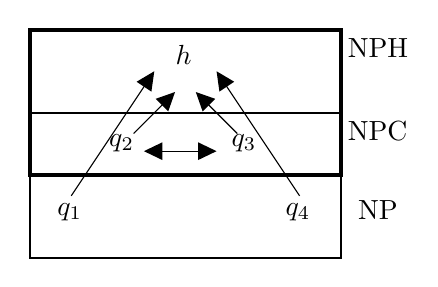
\begin{tikzpicture}[x=0.75pt,y=0.75pt,yscale=-1,xscale=1]
\draw  [line width=1.5]  (140,30) -- (290,30) -- (290,100) -- (140,100) -- cycle ;
\draw  [line width=0.75]  (140,70) -- (290,70) -- (290,140) -- (140,140) -- cycle ;
\draw    (210,88.5) -- (227,88.5) ;
\draw [shift={(230,88.5)}, rotate = 180] [fill={rgb, 255:red, 0; green, 0; blue, 0 }  ][line width=0.08]  [draw opacity=0] (8.93,-4.29) -- (0,0) -- (8.93,4.29) -- cycle    ;
\draw    (225,88.5) -- (198,88.5) ;
\draw [shift={(195,88.5)}, rotate = 360] [fill={rgb, 255:red, 0; green, 0; blue, 0 }  ][line width=0.08]  [draw opacity=0] (8.93,-4.29) -- (0,0) -- (8.93,4.29) -- cycle    ;

\draw    (160,110) -- (198.34,52.5) ;
\draw [shift={(200,50)}, rotate = 123.69] [fill={rgb, 255:red, 0; green, 0; blue, 0 }  ][line width=0.08]  [draw opacity=0] (8.93,-4.29) -- (0,0) -- (8.93,4.29) -- cycle    ;
\draw    (270,110) -- (231.66,52.5) ;
\draw [shift={(230,50)}, rotate = 56.31] [fill={rgb, 255:red, 0; green, 0; blue, 0 }  ][line width=0.08]  [draw opacity=0] (8.93,-4.29) -- (0,0) -- (8.93,4.29) -- cycle    ;
\draw    (190,80) -- (207.88,62.12) ;
\draw [shift={(210,60)}, rotate = 135] [fill={rgb, 255:red, 0; green, 0; blue, 0 }  ][line width=0.08]  [draw opacity=0] (8.93,-4.29) -- (0,0) -- (8.93,4.29) -- cycle    ;
\draw    (240,80) -- (222.12,62.12) ;
\draw [shift={(220,60)}, rotate = 45] [fill={rgb, 255:red, 0; green, 0; blue, 0 }  ][line width=0.08]  [draw opacity=0] (8.93,-4.29) -- (0,0) -- (8.93,4.29) -- cycle    ;

\draw (236,79.4) node [anchor=north west][inner sep=0.75pt]    {$q_{3}$};
\draw (177,79.4) node [anchor=north west][inner sep=0.75pt]    {$q_{2}$};
\draw (292,33) node [anchor=north west][inner sep=0.75pt]   [align=left] {NPH};
\draw (292,73) node [anchor=north west][inner sep=0.75pt]   [align=left] {NPC};
\draw (297,111) node [anchor=north west][inner sep=0.75pt]   [align=left] {NP};
\draw (262,112.4) node [anchor=north west][inner sep=0.75pt]    {$q_{4}$};
\draw (152,112.4) node [anchor=north west][inner sep=0.75pt]    {$q_{1}$};
\draw (209,36.15) node [anchor=north west][inner sep=0.75pt]    {$h$};
\end{tikzpicture}

\subsection{Complejidad Espacial}
Se utiliza como otra forma de clasificar problemas, según su dificultad computacional.

El modelo matemático para esta clasificación es la MT.

La complejidad espacial de una MTD M, que para siempre, es una función $f: N \rightarrow N$, tal que $f(n)$ es el máximo número de celdas que M visita para una entrada de longitud n.

Cantidad de espacio (memoria) que se requiere. El espacio a diferencia del tiempo se puede reutilizar.

Se dice que M se ejecutara en un espacio $f(n)$:
\begin{itemize}
  \item Ejem: $<MTD, w>$ MTD se ejecuta en $f(n)=4n$ para $n=2$ $f(2)=8$. Con entrada 2 usará un total de 8 celdas. 
\end{itemize}

\textbf{SPACE(f(n)):} Problemas (Lenguajes) decidibles por una MT Determinista (de una sola cinta) en ESPACIO POLINÓMICO. $PSPACE=\bigcup_k SPACE(n^k)$

\textbf{NSPACE(f(n)):} Problemas (Lenguajes) decidibles por una MT NO Determinista (de una sola cinta) en ESPACIO POLINÓMICO. $NPSPACE=\bigcup_k NSPACE(n^k)$

SAT por ejemplo es $O(n)$ en cuanto a espacio y en tiempo es exponencial.

\subsubsection{Teorema de Savitch (1970)}
$\forall f: N \rightarrow R^+$, donde $f(n)\geq n$. $\textit{NSPACE}(f(n)) \subseteq \textit{SPACE}(f^2(n))$

En otras palabras, cualquier problema decidible en una máquina de Turing no determinista en el espacio $f(n)$ también se puede decidir en una máquina de Turing determinista en el espacio $f^2(n)$.

Corolario: $\textit{PSPACE}(n^k)=\textit{NPSPACE}(n^k)$. Como los PSPACE absorben los NPSPACE resultan ser lo mismo.
\begin{itemize}
  \item $P \subseteq NP$. P incluido en NPC
  \item $P \subseteq \textit{PSPACE}$
  \item $NP \subseteq \textit{NPSPACE}$
  \item $\textit{PSPACE} = \textit{NPSPACE}$
  \item $P \subseteq NP \subseteq \textit{PSPACE}=\textit{NPSPACE} \subseteq \textit{EXPTIME}$
\end{itemize}